\documentclass[12pt]{article}
\usepackage[utf8]{inputenc}
\usepackage{amsmath, amsfonts, amssymb}
\usepackage[a4paper, margin=1in]{geometry}
\usepackage{varwidth}
\usepackage{graphicx}

\title{Random Variables and Stochastic Process (AI5030)}
\author{Soumyajit Chatterjee\\AI22MTECH02005 }


\begin{document}

\maketitle

\section*{Question 118 Dec (2017)}
Twenty items are put in a life testing experiment starting at time 0. The failure times of the items are recorded in a sequential manner. The experiment stops if all the twenty items fails or a pre-fixed time T$\geqslant 0$ is reached, whichever is earlier. If the lifetimes of the items are independent and identically distributed exponential random variables with mean $\theta$, where $0 < \theta < 10$, then which of the following statements are correct ?\\

\noindent 1. The MLE of $\theta$ always exists.

\noindent 2. The MLE of $\theta$ does not exist.

\noindent 3. The MLE of $\theta$ is an unbiased estimator of $\theta$ if it exists.

\noindent 4. The MLE of $\theta$ is bounded with probability 1, if it exists.

\section*{Solution}
An exponentially distributed Random Variable is given by the equation:

\begin{equation}
    f(x,\lambda) = 
        \begin{cases}
        \lambda e^{- \lambda x} & \text{ for } x \geqslant 0\\
        0 & \text{ for } x < 0
        \end{cases}
\end{equation}
\\
\noindent The graph of exponential Random Variable plot is:

\begin{figure}[h]
    \centering
    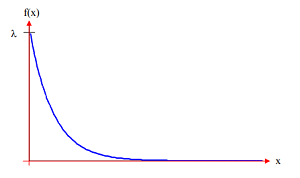
\includegraphics[width=0.5\textwidth]{exponential-distribution.png}
    \caption{Exponential Random Variable}
    \label{fig:erv}
\end{figure}

\clearpage
\noindent The CDF of exponential random variable is given by:

\begin{equation}
    F(x, \lambda) = ( 1 - e^{- \lambda x})
\end{equation}
\\
\noindent Here, the independent variable is time and mean $\theta$, therefore the CDF with respect to time t and mean $\theta$ is F(t, $\theta$) = (1 - $e^{- \theta t})$
\\

\noindent Out of the 20 items let the first item survive till time t$_1$ before failing.
\\

\noindent Therefore, the probability that the item survives till time t$_1$ before T where t is exponentially distributed is given by P(t $<$ T, $\theta)$ which is equal to the CDF of F(t$_1$, $\theta$).
\\

\noindent Therefore, the probability the item fails is given by 1 - F(t$_1$, $\theta$) which is 1 - (1 - e$^{-\theta t_1}$) = e$^{-\theta t_1}$
\\

\noindent Similarly, let the second item survive till time t$_2$ and the probability it survives till time t$_2$ is P(t$_2 <$ T, $\theta$) is given by the CDF F(t$_2$, $\theta$).
\\

\noindent Therefore, the probability the item fails is given by 1 - F(t$_2$, $\theta$) which is 1 - (1 - e$^{-\theta t_2}$) = e$^{-\theta t_2}$
\\

\noindent Therefore, the probability of all 20 items failing sequentially will be:

$$
P = e^{-\theta t_1}.e^{-\theta t_2}.e^{-\theta t_3}.e^{-\theta t_4}.e^{-\theta t_5}.e^{-\theta t_6}.....e^{-\theta t_{20}}
$$
\vspace{1mm}

\noindent Which will be equal to P$ = e^{-\theta ({t_1 + t_2 + t_3 + t_4 + ...... t_{20}})}$ , writing $t_1 + t_2 + t_3 + t_4 + ...... t_{20}$ as some constant $\tau$, we can rewrite the value of P$ = e^{-\theta \tau}$.
\\

\noindent From the definition of maximum likelihood estimation, we have to find that value of $\theta$ in the range $0 < \theta < 10$ that maximizes the probability P.
\\

\noindent To find the maximum value of the likelihood with respect to $\theta$ we can calculate $\dfrac{dP}{d\theta}$ = 0 to find the value of $\theta$ that maximizes P.
\\

\noindent However, P = e$^-\theta \tau$ is an exponential function, its derivative is also an exponential function which will never be exactly equal to 0. 
\\

\noindent Therefore, since $\dfrac{dP}{d\theta}$ will not be zero for any $\theta$, we cannot find the optimal $\theta$ that maximizes P. Therefore, the MLE for this problem does not exist.
\\

\noindent Therefore, option (2) is the correct option.

\end{document}